\documentclass{acm_proc_article-sp}
\usepackage{float}
\usepackage[british]{babel}
\usepackage{booktabs}
\usepackage[square,numbers]{natbib}
\bibliographystyle{acm}

\begin{document}

\title{Investigating the Prevalence of Server Name Indication in the Current HTTPS Ecosystem}

\numberofauthors{3}
\author{
\alignauthor
Shaown Sarker\\
       \affaddr{NC State University}\\
       \email{ssarker@ncsu.edu}
\alignauthor
Tae Hyun Kim\\
       \affaddr{NC State University}\\
       \email{tkim13@ncsu.edu}
\alignauthor
Douglas Reeves\\
       \affaddr{NC State University}\\
       \email{reeves@ncsu.edu}
}

\date{}

\maketitle

\begin{abstract}

The original SSL protocol required that the server present its certificate without the knowledge of the domain name being contacted by the client. Due to this restriction, servers were prevented from supporting more than one domain per IP address. Because a server could only serve a single certificate per IP address, and each certificate could contain only a single Common Name. To overcome this two extensions to the X.509 certificate specifications and TLS protocol were developed - the Subject Alternate Names (SAN) list and the Server Name Indication (SNI). In this paper, we look into the support of the SNI extension to the TLS protocol in concurrent HTTPS websites. Our findings show that although SNI is a very capable solution for the single certificate per IP problem, most popular websites do not force the client to be SNI capable despite supporting SNI. We also show that websites with lesser traffic tend to have lesser support for SNI.

\end{abstract}

\section{Introduction}

Online, secure communication begins with end-to-end authentication. Secure Sockets Layer (SSL) and Transport Layer Security (TLS)\footnote{Although SSL is a predecessor of TLS, both uses the same certificate architecture. When we refer to certificates or SSL certificates, it applies to both.} provides authentication for HTTPS traffic on the web. Coupled with a Public Key Infrastructure (PKI), SSL/TLS provides verifiable identities via certificate chains and private communication via encryption. 

Key sharing in the web's PKI is facilitated by recent additions to the SSl protocol and extensions to X.509 certificates. An SSL certificate is a signed binding between a subject and a public key. Certificate Authorities (CA) issue valid certificates, who themselves have their own certificates. This creates a logical chain of certificates - starting from a \textit{root} certificate through zero or more \textit{intermediate} certificates, to a \textit{leaf} certificate. In this chain, the certificate at a certain level is signed with the private key corresponding to the the certificate at the immediately previous level (with the sole exception of the root certificate, which is self-signed).

X.509~\cite{housley2002internet} is the most commonly used certificate management standard on the Internet. The certificates are commonly used as part of the SSL/TLS protocol (e.g., in HTTPS, IMAPS, etc). In SSL certificates, the subject is contained in the \textit{Common Name} field; for leaf certificates, the \textit{Common Name} is a domain name (e.g., \texttt{www.example.com}). SSL certificates also allow wildcard domains in the common name, so a certificate with a Common Name of *.example.com would cover both foo.example.com and bar.example.com. So, when a client contacts a server, it is essential that the domain name client is trying to contact is verified to be in the \textit{Common Name} of the certificate. Otherwise, the client should reject the connection as this could be the result of a possible interception (e.g., man-in-the-middle attacks).

Due to the design of the original SSL protocol, the server was required to present the certificate without knowing which domain name the client was contacting. This effectively prevented servers from supporting more than one domain per IP address, as a server could only serve a single certificate per IP address, and each certificate could contain only a single \textit{Common Name}. As a result, two extensions to the X.509 certificate specification and TLS protocol were developed:

\textbf{SAN list} - The Subject Alternate Names (SAN) extension allows a certificate to specify multiple alternate domain names to which the certificate should apply, effectively allowing a certificate to have multiple \textit{Common Names}. For example, a certificate with a SAN list \texttt{[*.google.com, *.youtube.com]} would be accepted for both \texttt{www.google.com} and \texttt{m.youtube.com}.

\textbf{SNI} - The Server Name Indication extension to the TLS protocol allows a client to specify which domain it is trying to contact before the server presents its certificate. If both the client and the server support SNI, this allows the server to host SSL certificates for different domains on a single IP address; the server simply examines the SNI field to select which certificate it should send to the client.

Popular websites now commonly use hosting providers for distributing content and mitigating denial-of-service attack~\cite{Holz:2011:SLT:2068816.2068856}. Websites are using third-party providers to host HTTPS content, but unfortunately, limitations of the TLS protocols have made this challenging for hosting providers. TLS has historically assumed that a given IP address would be used to host only a single website's domains, and that therefor it would suffice for any given IP address to server a single certificate. To support multiple customers' HTTPS content, hosting providers use one or more of the following approaches:
\begin{itemize}
\item \textbf{One customer per IP address} - The most straightforward approach involves having a single customer’s certificate (possibly with multiple domains in a SAN list) allocated to any given IP address. This has the benefit of not requiring clients to support SNI, but comes at a high monetary cost, as IPv4 addresses have grown more scarce.
\item \textbf{Cruise-liner certificates} - Finally, if a hosting provider can obtain custom certificates on behalf of its customers~\cite{Liu:2015:EMC:2815675.2815685}, it can craft certificates with SAN lists containing domains from multiple distinct customers. The problem with these "Cruise-liner" certificates is that the certificates cannot be modified piecemeal; adding or removing any customer's domain requires generating an entirely new certificate.
\item \textbf{Multiple certificates per IP address} - Hosting providers can host multiple certificates on any given IP address by using SNI. This is less expensive than dedicating an IP address to a single customer, but unfortunately older clients like Internet Explorer on Windows XP and Android 2.x devices do not support SNI. Thus, hosting providers are often hesitant to implement a solution that leaves these clients unable to access customer websites.

Although there have been research into overcoming this limitation of certificate on hosting providers using SAN list and cruise-liner certificate strategy~\cite{Cangialosi:2016:MAP:2976749.2978301}, there has not been much exploration of the SNI adoption over the HTTPS ecosystem. In this paper, we look into the SNI support over most popular websites in the Internet. Our research questions in this paper are:

\textbf{\textit{RQ1}} What is the current status of support for SNI over the most visited websites in the Internet?

\textbf{\textit{RQ2}} Is there any relationship between the amount of web traffic and SNI support?
\end{itemize}

The rest of the paper is organized as follows: section~\ref{sec:method} describes the methodology we used to answer our research questions, section~\ref{sec:res} discusses our findings and the answers to the research questions posited here, section~\ref{sec:relw} describes the literature related to our work, and we conclude in section~\ref{sec:conc} by reiterating our findings.

\section{Methodology} \label{sec:method}

As more e-commerce sites emerge and more businesses begin to store or share sensitive documents online, the ability to host and extend secure sites is becoming increasingly important. In the old-fashioned versions, there were two issues that had to be addressed in order to host a secure site:
\begin{itemize}
\item \textbf{SSL Scalability}: In multi-user environments such as shared hosting, because the number of secure sites that can be hosted on a server is limited, the site density finally had to be low.~\footnote{SSL Scalability. https://www.iis.net}
\item \textbf{IPv4 shortage}: Because the network endpoint can be identified only by the IP:Port binding, if the user wants to use the standard SSL port 443, each IP address must occasionally be assigned per user to host the secure site.
\end{itemize}

Also, Virtual hosting using SAN lists is both a fatal advantage and a weakness. They should  use the same certificate and key within only one server. Therefore, SAN list does not provide any solution for the following situations:
\begin{itemize}
\item Because the domain owner is different, user can not obtain an integrated key for domains owned by others from CA.
\item Even if the authority is delegated from the owner, the delegated administrator can misuse the issued key.
\item Or they can delegate key management to each person for each domain.
\end{itemize}

SNI offers a more fundamental solution to these problems. Server Name Indication (SNI) is a TLS extension that can include virtual domains as part of the TLS negotiation process. The practical implication of this is that now you can use the virtual domain name or host name to identify the network endpoint. In addition, a new highly scalable Web Hosting repository to support SNI is provided. As a result, the security site density is much higher, and nevertheless only uses one IP address.

However, using SNI requires the client to support SNI. Most new browsers support SNI, but IE in Windows XP, and android 2.x doesn't support SNI. Based on these limitations, we categorize the support for SNI into following three categories to answer our research questions:
\begin{itemize}
\item \textbf{Support SNI} - The server is capable of servicing requests from SNI supporting clients and will perform the certificate exchange.
\item \textbf{Requires SNI} - The server supports SNI, but requires that the client presents the domain name it is trying to contact beforehand, otherwise the server presents with a default certificate and will not perform the domain specific certificate exchange.
\item \textbf{Forces SNI} - The server does not perform the certificate exchange at all without the client presenting the domain name it is trying to contact.
\end{itemize}

The second and third category are a subset of the first category. To determine whether the website server has SNI capabilities as categorized above, we used the open-source tool openssl~\footnote{https://www.openssl.org/}. OpenSSL comes with a client tool that can connect to a secure server. The tool is similar to telnet or nc, in the sense that it handles the SSL/TLS layer but allows the user to fully control the layer that comes next.

To connect to a server, we need to supply a host-name and a port~\cite{ristic2013openssl}. For example:

\texttt{\$ openssl s\_client -connect www.feistyduck.com:443}

To have SNI enabled in \texttt{s\_client}, we need to use the \texttt{s\_client} with the \texttt{-servername} switch~\cite{ristic2013openssl}:

\texttt{\$ openssl s\_client -connect www.feistyduck.com:443 -servername www.feistyduck.com}

Both of these command initiates the certificate exchange and we receive the certificate from the server. Based on the response from the website server from these two commands, we define our SNI support categories as follows:
\begin{itemize}
\item \textbf{Support SNI} - The server performs a certificate exchange with the \texttt{-servername} switch and we have a certificate from the server.
\item \textbf{Requires SNI} - The server performs certificate exchange for both with and without the \texttt{-servername} switch, but the certificates are different, thus indicating that the server requires an SNI capable client for proper HTTPS communication.
\item \textbf{Forces SNI} - The server performs a certificate exchange for only with \texttt{-servername} switch and we receive no certificate for a default connection.
\end{itemize}

To answer our research questions, we also retrieved the list of top 1 million websites~\footnote{http://s3.amazonaws.com/alexa-static/top-1m.csv.zip} ranked by web-traffic published by Alexa~\footnote{www.alexa.com}. Using the openssl tool, we collected the SNI support information fro the top 150,000 ranked websites along with the respective default and SNI certificates into a MySql database. Due to the geophysical location of the website host providers and their latency, we added a timeout of 10 seconds, so that if the certificate exchange does not take place between the 10 seconds from the start of the connect request, it is aborted.

\section{Results} \label{sec:res}
Using our collected data we answer our research questions as follows:

\textbf{\textit{RQ1}} What is the current status of support for SNI over the most visited websites in the Internet?

We divided our data over rank ranges of 25,000 dividing into 6 ranges. Over these ranges, we measured the number of website server that supports, requires, and force SNI, which is depicted in figure~\ref{fig:sranks}. We can see that although SNI support is considerably high, a much smaller number of websites requires SNI and even a smaller number of websites actually forces SNI requirement upon clients. We can attribute this to the website host providers tendency to support SNI, but not denying service to legacy clients.

\begin{figure}[htbp]
\center
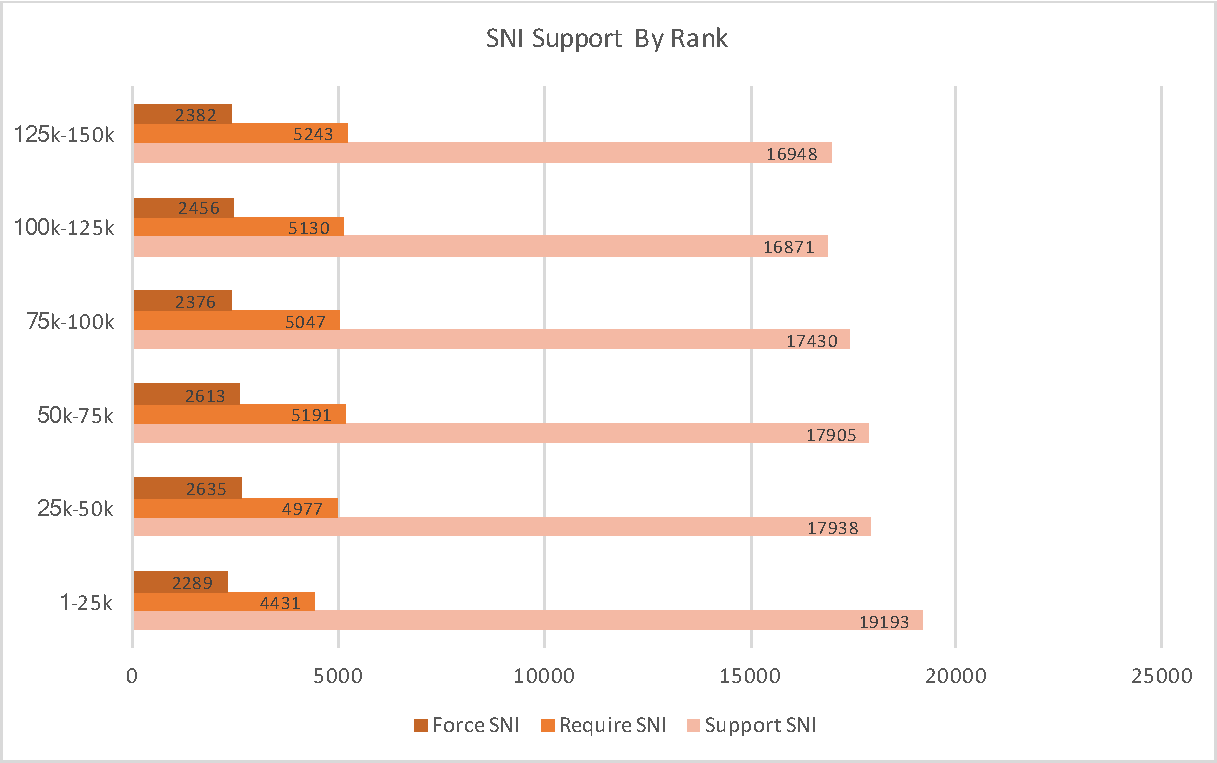
\includegraphics[width=0.5\textwidth]{by_rank_ranges}
\caption{SNI Support by Ranks}
\label{fig:sranks}
\end{figure}

\textbf{\textit{RQ2}} Is there any relationship between the amount of web traffic and SNI support?

To answer this question, we looked at the SNI support throughout the ranks in a cumulative manner, this is presented in table~\ref{tab:pranks}. From this data, we can see that none of the top 100 websites forces SNI upon the clients, and a very small number of websites requires SNI; although there is almost ubiquitous SNI support among the top 100 websites.

% Table generated by Excel2LaTeX
\begin{table}[htbp]
  \centering
  \caption{SNI Support over Cumulative Ranks}
    \begin{tabular}{l|r|r|r}
    \toprule
    \multicolumn{1}{l}{Rank Range} & \multicolumn{1}{l}{Support SNI} & \multicolumn{1}{l}{Require SNI} & \multicolumn{1}{l}{Force SNI} \\
    \midrule
    <=100 & 97    & 25    & 0 \\
    <=1k  & 872   & 158   & 34 \\
    <=5k  & 4108  & 749   & 298 \\
    <=10k & 8028  & 1658  & 774 \\
    <=20k & 15525 & 3504  & 1786 \\
    <=50k & 37131 & 9408  & 4924 \\
    \midrule
    Overall & 106285 & 30019 & 14751 \\
    \bottomrule
    \end{tabular}%
  \label{tab:pranks}%
\end{table}%

Figure~\ref{fig:pranks} shows the data in table~\ref{tab:pranks} as a percentage representation. From the data we can see that, as we move into lower ranked websites the support for SNI decreases, and at the same time we see a minute but steady increase in the require and force SNI categories. We can explain this observation in terms of website traffic. As the high volume websites desire to reach the wider set of clients, they tend not to force clients to have SNI capabilities, but lower volume traffic sites are often hosted by providers requiring or forcing SNI due to lowering of infrastructure and maintenance cost, as SNI enables the hosting provider to have multiple certificates per IP, but at the same time denying legacy clients of the server.

\begin{figure}[htbp]
\center
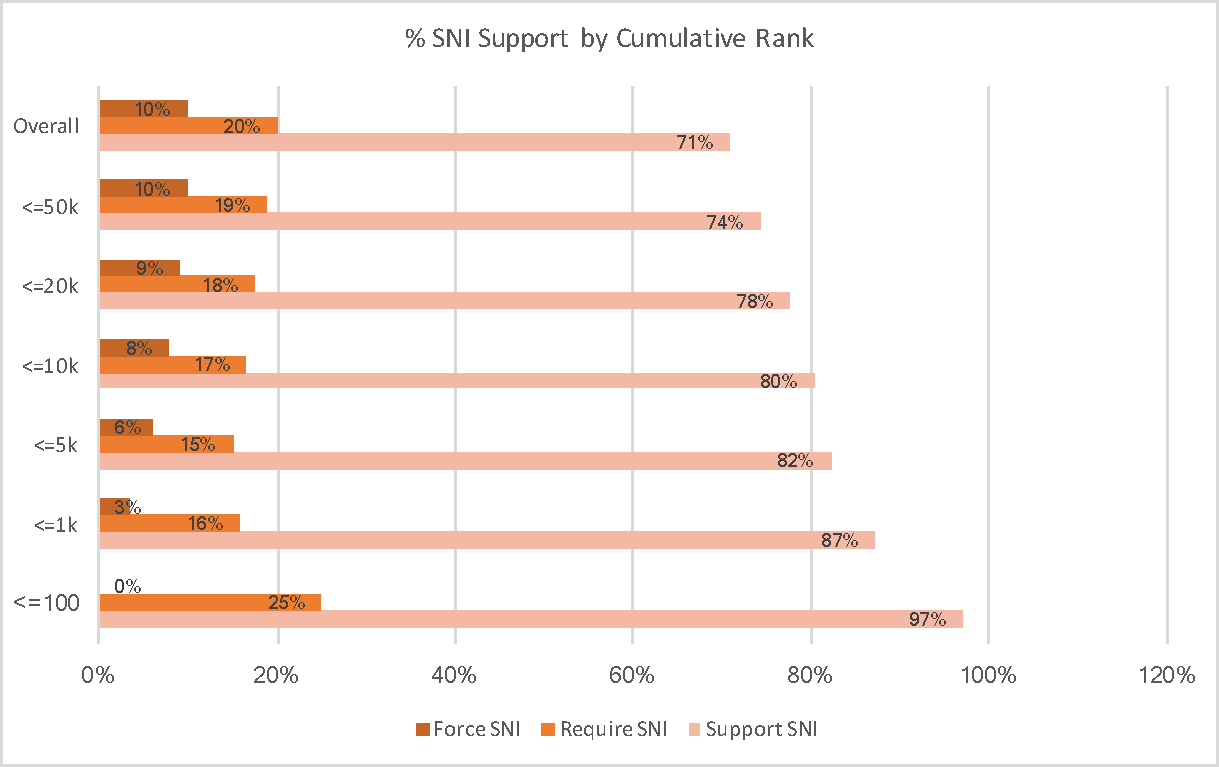
\includegraphics[width=0.5\textwidth]{by_incremental_ranks}
\caption{Percent of SNI Support by Cumulative Rank}
\label{fig:pranks}
\end{figure}

\section{Related Work} \label{sec:relw}
Cangialosi et al. in their 2016 work~\cite{Cangialosi:2016:MAP:2976749.2978301} looks into the private key sharing in the HTTPS ecosystem. They focus on the nature of key sharing between website hosting providers and the CDNs, certificate reissues and revocation as managed by third party providers, and the trust between organizations and their third party counterpart. In their work, the authors measure the number of certificates per IP based on the SAN list extension and cruise-liner certificate management through crafting custom certificates SAN lists. Our work extends on the work by Cangialosi et al. by exploring the other extension to TLS protocol - SNI and it's usage in the current HTTPS ecosystem.

Recent work by Liang et al. explores how Content Delivery Networks (CDN) manage SSL certificates when distributing HTTPS content to the customers~\cite{Liu:2015:EMC:2815675.2815685}. They observe the distinction between custom and shared certificates, many instances of mismanagement, CAs neglecting to revoke certificates, and private key sharing. They specifically look into cruise-liner certificates. Our work compliments the work by Liang et al. by looking into the other prominent strategy available to overcome the shortcoming of a single certificate per IP. 

There also have been numerous work on understanding and improving the SSL certificate ecosystem through measurements of CAs~\cite{Durumeric:2013:AHC:2504730.2504755,Zhang:2014:ASC:2663716.2663758,laurie2013certificate}, and  measurements of the cost of HTTPS security~\cite{naylor2014cost}. In contrast, our work builds upon these by focusing on the server level certificates and their exchange policies. We primarily focus on the issue of servers being limited to a single certificate per IP and how they tend to solve it through SNI while exploring the relationship between web-traffic and the SNI support.

\section{Conclusion} \label{sec:conc}

In our work, we investigated the prevalence of SNI support among the top websites in the Internet. Our findings show that the websites with most web-traffic volume tend to support SNI, but they rarely require or force their clients to be SNI capable. On the other hand, websites with lower volume of traffic, either are reserved in their support of SNI or tend to require or force SNI capable clients for ease of infrastructure setup and maintenance cost. To reiterate our contributions, we collected and analyzed the current status of SNI support among the top 150,000 websites in the Internet along with their respective default and SNI enabled certificates.

% include your own bib file like this:
\bibliography{refs}

\section*{Appendix}
All of our code along with the data is available under the MIT license in the Github repository: \texttt{https://goo.gl/ybtNrj}

\end{document}